\section{Bevezetés}
    A feladatkiírásban felvázolt probléma egy forgásszimmetrikus elrendezés, emiatt \aref{fig:elrendezes_2d}. ábrán látható fél-síkmetszet vizsgálata elég a probléma megoldásához.\\[1ex]

    \begin{wrapfigure}{L}{0.35\textwidth}
        \centering
        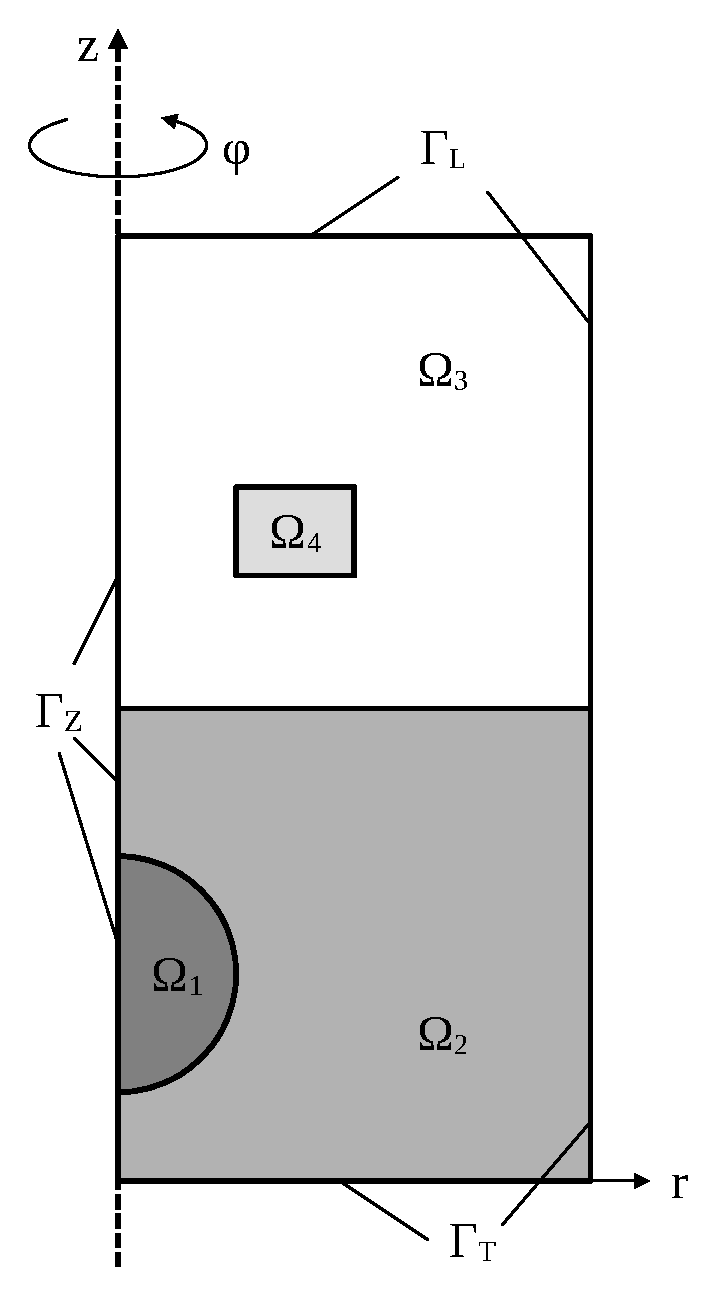
\includegraphics[width=0.9\linewidth]{elrendezes_2d.pdf}
        \caption{A szimulált elrendezés.}
        \label{fig:elrendezes_2d}
    \end{wrapfigure}

 A tartományok és határfelületek (határvonalak) jelentése:
    \begin{itemize}
        \item[$\Omega_1$] -- vasgömb
        \item[$\Omega_2$] -- talaj
        \item[$\Omega_3$] -- levegő
        \item[$\Omega_4$] -- tekercs
        \item[$\Gamma_Z$] -- szimmetriatengely
        \item[$\Gamma_L$] -- vizsgált levegővel kitöltött térrész határa
        \item[$\Gamma_T$] -- vizsgált talajjal kitöltött térrész határa
    \end{itemize}

    Mivel csak egy adott $\omega$ körfrekvencián kell vizsgálódnunk, emiatt elég a szinuszos állandósult állapottal foglalkoznunk.
    \begin{align}
        \dfrac{\partial \vec{B}}{\partial t} \quad&\longrightarrow\quad j\omega\vec{B}
    \end{align}
    A kérdéses $\omega$ körfrekvencián az elektromágneses hullámok szabadtéri hullámhossza (mert $\epsilon_r = 1$):
    \begin{align}
        \lambda &= \dfrac{c}{f} = \dfrac{c}{\dfrac{\omega}{2\pi}} = \dfrac{\qty{3e8}{\metre\per\second}}{\dfrac{2\pi\qty{500}{\per\second}}{2\pi}} = \qty{6e5}{\metre}
    \end{align}
    Emiatt $\lambda$ az \qty{1000}{km} nagyságrendjébe esik, míg az elrendezés fizikai méretei néhányszor \qty{10}{cm}-esek, így élhetünk a magneto-kvázistacionárius közelítéssel:
    \begin{align}
        \dfrac{\partial \vec{D}}{\partial t} \quad&\longrightarrow\quad 0
    \end{align}
    \clearpage
    Ebben az esetben a vizsgált tartományon belül a Maxwell-egyenleteknek a következő alakja érvényes:
    \begin{align}
        \rot \vec{H} &= \vec{J} \\
        \rot \vec{E} &= -j\omega\vec{B}\\
        \divergence \vec{B} &= 0\\
        \vec{B} &= \mu\vec{H}\\
        \vec{J} &= \sigma \vec{E} + \vec{J}_i
    \end{align}

    \begin{align}
        \sigma(\vec{r}) &=
            \begin{cases}
                \sigma, & \text{ha } \vec{r} \in \Omega_1\\
                \sigma_t, & \text{ha } \vec{r} \in \Omega_2\\
                0, & \text{ha } \vec{r} \in \Omega_3 \cup \Omega_4
            \end{cases}
    \end{align}

    Az $R$ sugarat megfelelően nagyra kell választani ahhoz, hogy a kialakuló teret ne befolyásolja jelentősen a vizsgált $\Omega$ tartomány $\Gamma_T \cup \Gamma_L$ ,,távoli'' peremének a közelsége.
    
